%%%%%%%%%%%%%%%%%%%%%%%%%%%%%%%%%%%%%%%%%
% a0poster Portrait Poster
% LaTeX Template
% Version 1.0 (22/06/13)
%
% The a0poster class was created by:
% Gerlinde Kettl and Matthias Weiser (tex@kettl.de)
% 
% This template has been downloaded from:
% http://www.LaTeXTemplates.com
%
% License:
% CC BY-NC-SA 3.0 (http://creativecommons.org/licenses/by-nc-sa/3.0/)
%
%%%%%%%%%%%%%%%%%%%%%%%%%%%%%%%%%%%%%%%%%

\newcommand{\vcenteredinclude}[1]{\begingroup
    \setbox0=\hbox{\includegraphics[width=\linewidth]{#1}}%
\parbox{\wd0}{\box0}\endgroup}

%----------------------------------------------------------------------------------------
%	PACKAGES AND OTHER DOCUMENT CONFIGURATIONS
%----------------------------------------------------------------------------------------

\documentclass[a0,portrait]{a0poster}

\usepackage{multicol} % This is so we can have multiple columns of text side-by-side
\columnsep=100pt % This is the amount of white space between the columns in the poster
\columnseprule=3pt % This is the thickness of the black line between the columns in the poster

\usepackage[svgnames]{xcolor} % Specify colors by their 'svgnames', for a full list of all colors available see here: http://www.latextemplates.com/svgnames-colors

\usepackage[sc]{mathpazo}
\linespread{1.08}         % Palatino needs more leading (space between lines)

\usepackage{graphicx} % Required for including images
\usepackage{booktabs} % Top and bottom rules for table
\usepackage[font=normalsize,labelfont=sc]{caption} % Required for specifying captions to tables and figures
\usepackage{amsfonts, amsmath, amsthm, amssymb} % For math fonts, symbols and environments
\usepackage{wrapfig} % Allows wrapping text around tables and figures
\usepackage[utf8]{inputenc} 
\usepackage[detect-all]{siunitx}
\usepackage[T1]{fontenc}
\usepackage{authblk}
\usepackage{enumitem}
\usepackage[sc]{titlesec}

\setdescription{leftmargin=\parindent,labelindent=4\parindent}

% Remove the author and date fields and the space associated with them
% from the definition of maketitle!
\makeatletter
\renewcommand{\@maketitle}{
\newpage
 \null
 \vskip 2em%
 \begin{center}%
  {
 \veryHuge \color{NavyBlue} \@title \par}%
 \end{center}%
 \par} \makeatother
%\preauthor{\huge}
%\postauthor{\par \vspace{2cm}
    %\Large\texttt{matteo.abis@psi.ch}}

%\renewcommand\Affilfont{\Large}
\renewcommand{\labelitemi}{$\vcenter{\hbox{\tiny$\bullet$}}$}
\newenvironment{spacedcenter}{
    \vspace{2cm}\begin{center}}
        {\end{center}
    \vspace{2cm}\par}

\setlength{\parindent}{0cm}

\title{Phase-contrast imaging on lab sources}

\begin{document}

%----------------------------------------------------------------------------------------
%	POSTER HEADER 
%----------------------------------------------------------------------------------------

% The header is divided into two boxes:
% The first is 75% wide and houses the title, subtitle, names, university/organization and contact information
% The second is 25% wide and houses a logo for your university/organization or a photo of you
% The widths of these boxes can be easily edited to accommodate your content as you see fit
\maketitle

\thispagestyle{empty}

\vspace{1\baselineskip}

\centering
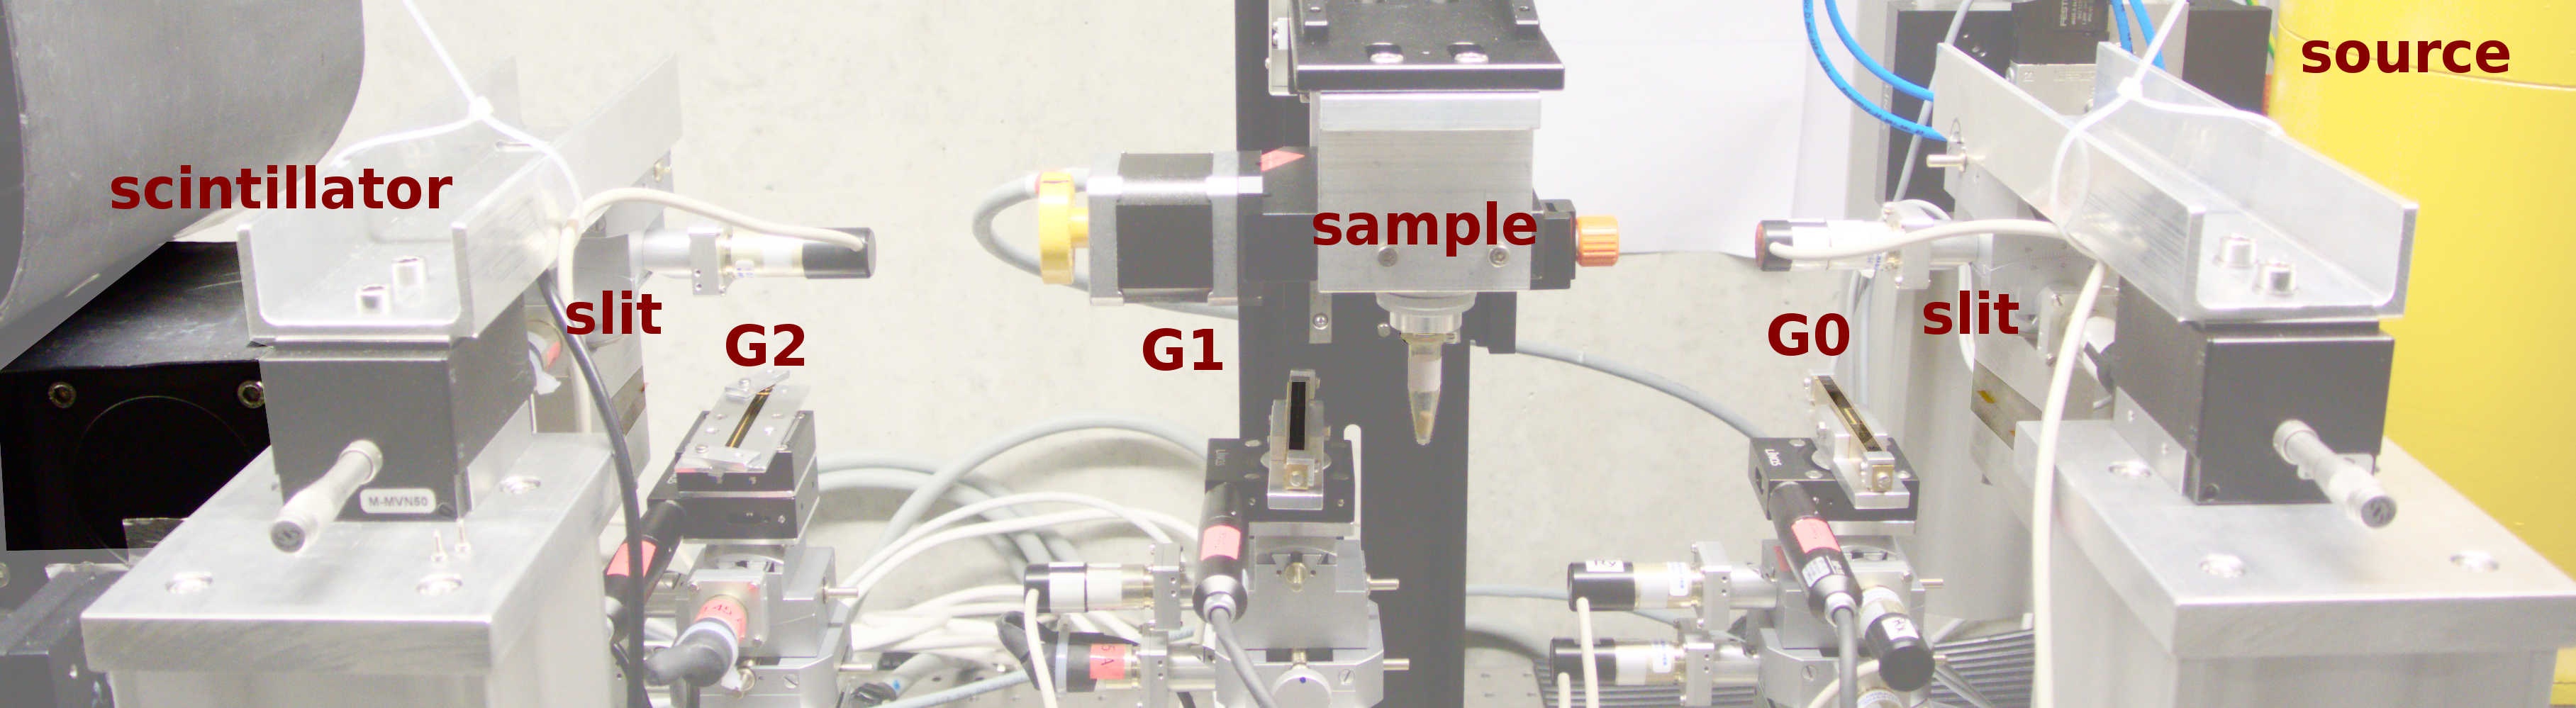
\includegraphics[width=\textwidth]{side.png}

\vspace{2\baselineskip} % A bit of extra whitespace between the header and poster content

\begin{minipage}[b]{0.58\linewidth}
    \vcenteredinclude{line.png}
\end{minipage}
\hspace*{\fill}
\begin{minipage}[b]{0.2\linewidth}
    \huge
    \vspace*{\fill}
\begin{tabular}{ll}
    \multicolumn{2}{c}{High-energy setup}\\[.5\baselineskip]
    \midrule
    \textbf{design energy} & $\SI{120}{\kilo\eV}$ \\
    \textbf{total length} & \SI{83}{\centi\metre} \\
    \textbf{Talbot order} & 1\\
    \textbf{field of view} & \SI{2.5}{\centi\metre}\\
\end{tabular}
    \vspace*{\fill}
\end{minipage}
\hspace*{\fill}

\vspace{2\baselineskip} % A bit of extra whitespace between the header and poster content
\noindent\rule{\textwidth}{2pt}

\vspace{2\baselineskip} % A bit of extra whitespace between the header and poster content
\includegraphics[width=\textwidth]{Figure1_V1.jpg}
%----------------------------------------------------------------------------------------
\end{document}
